% Options for packages loaded elsewhere
\PassOptionsToPackage{unicode}{hyperref}
\PassOptionsToPackage{hyphens}{url}
%
\documentclass[
  10pt,
]{book}
\usepackage{amsmath,amssymb}
\usepackage{iftex}
\ifPDFTeX
  \usepackage[T1]{fontenc}
  \usepackage[utf8]{inputenc}
  \usepackage{textcomp} % provide euro and other symbols
\else % if luatex or xetex
  \usepackage{unicode-math} % this also loads fontspec
  \defaultfontfeatures{Scale=MatchLowercase}
  \defaultfontfeatures[\rmfamily]{Ligatures=TeX,Scale=1}
\fi
\usepackage{lmodern}
\ifPDFTeX\else
  % xetex/luatex font selection
    \setmainfont[Numbers=OldStyle]{Charis SIL}
  \newfontfamily{\arabicfont}[Script=Arabic,Scale=1.0]{Vazirmatn-Light}
  \newfontfamily{\tradarab}[Script=Arabic,Scale=1.0]{Amiri}
  \newfontfamily{\tradarabsmall}[Script=Arabic,Scale=0.75]{Amiri}
\fi
% Use upquote if available, for straight quotes in verbatim environments
\IfFileExists{upquote.sty}{\usepackage{upquote}}{}
\IfFileExists{microtype.sty}{% use microtype if available
  \usepackage[]{microtype}
  \UseMicrotypeSet[protrusion]{basicmath} % disable protrusion for tt fonts
}{}
\makeatletter
\@ifundefined{KOMAClassName}{% if non-KOMA class
  \IfFileExists{parskip.sty}{%
    \usepackage{parskip}
  }{% else
    \setlength{\parindent}{0pt}
    \setlength{\parskip}{6pt plus 2pt minus 1pt}}
}{% if KOMA class
  \KOMAoptions{parskip=half}}
\makeatother
\usepackage{xcolor}
\usepackage[paperwidth=156mm,paperheight=234mm,bindingoffset=16mm,textwidth=114.8mm,textheight=170.8mm,twoside]{geometry}
\usepackage{longtable,booktabs,array}
\usepackage{calc} % for calculating minipage widths
% Correct order of tables after \paragraph or \subparagraph
\usepackage{etoolbox}
\makeatletter
\patchcmd\longtable{\par}{\if@noskipsec\mbox{}\fi\par}{}{}
\makeatother
% Allow footnotes in longtable head/foot
\IfFileExists{footnotehyper.sty}{\usepackage{footnotehyper}}{\usepackage{footnote}}
\makesavenoteenv{longtable}
\usepackage{graphicx}
\makeatletter
\def\maxwidth{\ifdim\Gin@nat@width>\linewidth\linewidth\else\Gin@nat@width\fi}
\def\maxheight{\ifdim\Gin@nat@height>\textheight\textheight\else\Gin@nat@height\fi}
\makeatother
% Scale images if necessary, so that they will not overflow the page
% margins by default, and it is still possible to overwrite the defaults
% using explicit options in \includegraphics[width, height, ...]{}
\setkeys{Gin}{width=\maxwidth,height=\maxheight,keepaspectratio}
% Set default figure placement to htbp
\makeatletter
\def\fps@figure{htbp}
\makeatother
\setlength{\emergencystretch}{3em} % prevent overfull lines
\providecommand{\tightlist}{%
  \setlength{\itemsep}{0pt}\setlength{\parskip}{0pt}}
\setcounter{secnumdepth}{5}
\ifLuaTeX
\usepackage[bidi=basic]{babel}
\else
\usepackage[bidi=default]{babel}
\fi
\babelprovide[main,import]{english}
\ifPDFTeX
\else
\babelfont{rm}[Numbers=OldStyle]{Charis SIL}
\fi
\babelprovide[import]{arabic}
% get rid of language-specific shorthands (see #6817):
\let\LanguageShortHands\languageshorthands
\def\languageshorthands#1{}
\newcommand{\gitTag}{\input|"git describe"}
\usepackage{lipsum}
\usepackage{metalogo}
\usepackage{xcolor}
\usepackage{url}
\usepackage{fancyhdr}

% To use New Computer Modern font, uncomment following two lines only
%\defaultfontfeatures{Numbers=OldStyle} % have to load this first, before loading fontsetup
%\usepackage[default]{fontsetup} % "default" option loads book weight.
%\addfontfeature{Numbers=Lowercase} % don't need this

% section style, all section headings normal size
\usepackage{sectsty}
\allsectionsfont{\normalsize}


% section style, all section headings normal size bold, except chapter headings
\usepackage[bf,tiny]{titlesec}
%\definecolor{gray75}{gray}{0.5}
%\titleformat*{\chapter}      {\normalfont\normalsize\color{gray75}}
%\titleformat*{\section}      {\normalfont\normalsize\color{gray75}}
%\titleformat*{\subsection}   {\normalfont\normalsize\color{gray75}}
%\titleformat*{\subsubsection}{\normalfont\normalsize\color{gray75}}

% Arabic font's ascenders, descenders, and diacritics increase Latex's line
% spacing irregularly for some lines more than others to result in a visually
% unappealing output.
%
% I tried setting \lineskiplimit=-\maxdimen as some had suggested this but it
% completely destroys linespacing in tables and around tikzpictures.
%
% Then I found that \smash forces a 0 depth and 0 height for it's argument. So
% the Arabic text is ignored by Latex for line spacing purposes. Call \smash on
% the Arabic text input to babel's \foreignlanguage as below.
%
% I also tried calling smash on the output of \foreignlanguage but that seemed
% to cause problems on chapter headings.
%
% However, with this solution, some itemized lists have Arabic text directly on
% top of each other and the diacritics collide. For these lists insert a
% \vphantom{\huge J} for each item to locally increase line spacing. See
% examples in script.Rmd and inna_and_its_sisters.Rmd.
%
% The other unsolved issue with the solution is that it messes up the bidi dir
% in the sidebar contents in my PDF reader
\AddBabelHook[arabic]{smash}{foreign}{\def\BabelText##1{\smash{##1}}}

% Add section symbol § to every (sub)section heading and reference
%\NewCommandCopy{\oldthesection}{\thesection}
%\renewcommand{\thesection}{\S\oldthesection}

% Fancy header

% use this command from preface
%\newcommand{\forcefancyhdr}[1]{\markboth {\textsc{\MakeLowercase{#1}}}{\textsc{\MakeLowercase{#1}}}}

\renewcommand{\chaptermark}[1]{\markboth {\textsc{\MakeLowercase{\scalebox{1}[0.81]{\thechapter}\ #1}}}{}}
\renewcommand{\sectionmark}[1]{\markright{\textsc{\MakeLowercase{\scalebox{1}[0.81]{\S\thesection}\ }}}}

% Start fancy header style beginning here, override with thispagestyle{empty} for copyright page
\pagestyle{fancy}

\fancypagestyle{mymainstyle}{%
\fancyhf{}
%\fancyhead[LE]{\thepage\phantom{xxx}\itshape\nouppercase{Fundamentals of Standard Arabic}}
%\fancyhead[RO]{\itshape\nouppercase{\leftmark}\phantom{xxx}\thepage}
%\fancyhead[LE]{\thepage \ {\vrule height 13pt width 1pt} \itshape\nouppercase{Fundamentals of Standard Arabic}}
%\fancyhead[RO]{\itshape\nouppercase{\leftmark} \ {\vrule height 13pt width 1pt} \thepage}

%\fancyhead[LE]{\leavevmode\smash{\llap{\thepage\ \rule[-0.5em]{1pt}{1.5em}}}\phantom{x}\itshape\nouppercase{Fundamentals of Standard Arabic}}
%\fancyhead[RO]{\textsl{\nouppercase{\leftmark}}\phantom{x}\leavevmode\smash{\rlap{\rule[-0.5em]{1pt}{1.5em}\ \thepage}}}
%\fancyhead[LO]{\itshape\nouppercase{\rightmark}}
%\fancyhead[LO,RE]{\textsl{\nouppercase{https://adamiturabi.github.io/arabic-tutorial-book/}}}

% Put page numbers outside text block in top margin
%\fancyhead[LE]{\hspace*{-1cm}\thepage}
%\fancyhead[RO]{\thepage\hspace*{-1cm}}

% Put page numbers inside text block in top margin
\fancyhead[LE,RO]{\scalebox{1}[0.81]{\thepage}}

\fancyhead[CO]{\nouppercase{\rightmark}}
\fancyhead[CE]{\nouppercase{\leftmark}}
\renewcommand{\headrulewidth}{0pt}

\fancyfoot[RE, RO]{\phantom{xxx}\\\phantom{xxx}\\\phantom{xxx}\\\phantom{xxx}\\\textcolor{gray}{\tiny{Author Names, \textit{Learn Standard Arabic}, \texttt{\gitTag}\\\url{https://adamiturabi.github.io/arabic-tutorial-book/}}}}

}% definition of mymainstyle

% Footer for chapter start pages:
\fancypagestyle{plain}{%
\fancyhf{}
\fancyfoot[RE, RO]{\phantom{xxx}\\\phantom{xxx}\\\phantom{xxx}\\\phantom{xxx}\\\textcolor{gray}{\tiny{Author Names, \textit{Learn Standard Arabic}, \texttt{\gitTag}\\\url{https://adamiturabi.github.io/arabic-tutorial-book/}}}}
\fancyfoot[CO]{\scalebox{1}[0.81]{\thepage}}
}

% Blank pages (e.g., left hand pages between chapters should be completely blank. no headers even
\makeatletter
\def\cleardoublepage{\clearpage\if@twoside \ifodd\c@page\else
  \begingroup
    \mbox{}
    \vspace*{\fill}
    \begin{center}
      %This page intentionally contains only this sentence.
    \end{center}
    \vspace{\fill}
    \thispagestyle{empty}
    \newpage
    \if@twocolumn\mbox{}\newpage\fi
  \endgroup\fi\fi}
\makeatother

\usepackage[color={[gray]{0.85}}, fontsize=32pt, text={Work in progress. Not ready for study.}]{draftwatermark}

\widowpenalty10000
%\clubpenalty10000

\babelfont[arabic]{rm}
          [Language=Default]{Vazirmatn-Light}
\babelfont[arabic]{sf}
          [Language=Default]{Vazirmatn-Light}

% Customize ToC table of contents
\usepackage[titles]{tocloft}

% Reserve horizontal spacing for chapter and section numbers
\setlength{\cftchapnumwidth}{3em}
\setlength{\cftsecnumwidth}{3em}

% No dots between chapter/section name and page number
\renewcommand{\cftchapdotsep}{\cftnodots}
\renewcommand{\cftsecdotsep}{\cftnodots}

% Some horizontal space between chapter/section name and page number
\renewcommand{\cftchapleader}{\quad}
\renewcommand{\cftsecleader} {\quad}
\renewcommand{\cftchapafterpnum}{\cftparfillskip}
\renewcommand{\cftsecafterpnum}{\cftparfillskip}
% Page number aligned left instead of right
\renewcommand{\cftpnumalign}{l}

% Chapter and section name font sizes
\renewcommand\cftchapfont{\normalfont}
\renewcommand\cftsecfont{\footnotesize}

% Chapter and section page number font sizes
\renewcommand\cftchappagefont{\normalfont}
\renewcommand\cftsecpagefont{\footnotesize}

% Short/brief table of contents before detailed one
% See frontpage.tex for additional customization there
\usepackage[tight]{shorttoc}

% Change title of original ToC to contrast with shorttoc title
\addto\captionsenglish{% Replace "english" with the language you use
  \renewcommand{\contentsname}%
    {Detailed Contents}%
}
\ifLuaTeX
  \usepackage{selnolig}  % disable illegal ligatures
\fi
\usepackage{csquotes}
\usepackage{bookmark}
\IfFileExists{xurl.sty}{\usepackage{xurl}}{} % add URL line breaks if available
\urlstyle{same}
\hypersetup{
  pdftitle={Learn Standard Arabic},
  pdfauthor={Author Names},
  pdflang={en},
  hidelinks,
  pdfcreator={LaTeX via pandoc}}

\title{Learn Standard Arabic}
\usepackage{etoolbox}
\makeatletter
\providecommand{\subtitle}[1]{% add subtitle to \maketitle
  \apptocmd{\@title}{\par {\large #1 \par}}{}{}
}
\makeatother
\subtitle{A self-instruction textbook with grammar, vocabulary, and exercises}
\author{Author Names}
\date{v0.1.0-738-g3538b25}

\begin{document}
\maketitle

\thispagestyle{empty}
%% copyrightpage
\begingroup
\footnotesize
\parindent 0pt
\parskip \baselineskip
\textcopyright{} 2023 Author Names \\
All rights reserved.

    This work may not be distributed or modified, without written permission from the copyright holder.

%\begin{center}
%\begin{tabular}{ll}
\texttt{\gitTag}
%\end{tabular}
%\end{center}

This book is typeset with \XeLaTeX\ (via the R bookdown package and the pandoc document converter)
in the Charis, Vazirmatn, and Amiri typefaces.


\vfill


%%%%{\LARGE\plogo}
%\vspace*{2\baselineskip}


\endgroup
\clearpage

\newpage
% Force Latex to begin Main matter headers and pagination from the very beginning
%\mainmatter
\pagestyle{mymainstyle}
\begingroup
% For short ToC remove vertical spacing between lines for more condensed look
%\setlength{\cftparskip}{-2pt}
\setlength{\cftbeforechapskip}{-3pt}
\shorttableofcontents{Brief Contents}{0}
\endgroup


{
\setcounter{tocdepth}{1}
\tableofcontents
}
\chapter*{Preface}\label{preface}
\addcontentsline{toc}{chapter}{Preface}

\markboth {\textsc{\MakeLowercase{Preface}}}{\textsc{\MakeLowercase{Preface}}}

\begin{center}
\tradarab{
الرحيم
الرحمن
الله
بسم
}
\end{center}

The primary texts of Islām (the Qurʾān and the Ḥadīt͡h) are in Arabic. So too is much of its scholarly literature. However, there is a multitude of Muslims for whom Arabic is not a native language, yet who are familiar enough with English to study textbooks written in this language. The goal of this book is to help them learn Arabic at a beginner's level so that, together with a study of the appropriate expositional texts, they are one step closer to understanding the primary texts in their original language. We hope that this will, if Allāh wills, make them feel more connected to the primary texts and their teachings. Furthermore, they can be empowered to study the vast body of Arabic Islāmic literature.

This book is a teaching grammar and not a reference grammar. So, in the initial chapters, topics are presented sequentially at only a basic level, without treating them exhaustively, before moving on to the next topic. Furthermore, since this is a beginner's textbook, only the more common usages are explained.

We have also aimed to make this a self-instruction textbook so that a diligent student should, if Allāh wills, be able to study it without an instructor. The target learner is someone who has not been exposed to grammatical terminology like \emph{inflection}, \emph{case}, \emph{mood}, etc. While terminology is necessary for a rigorous non-immersive learning of language, we have tried to steer away from Latin-based terms like \emph{accusative} and \emph{jussive}. Such terms, when first encountered by an uninitiated learner, may deter from proceeding further. (Learning a language can be hard enough without getting the feeling that your grammar book is accusing you of something!) So we have in some places translated the meaning of Arabic grammar terms to English. In other places, we have used established English grammar terms where the terms are basic enough. We have even, in places, invented terms where we deemed appropriate. The drawback to this non-standard approach, however, is that the student may not be able to immediately relate the terminology he has learned in this book to established terminology in other grammar textbooks. To remedy this to some extent, we provide a glossary in the appendix which maps the grammatical terminology used in this book to other, established, Latin-based and Arabic-based counterparts.

It may also be appropriate to inform the reader that we chose to present a simplified version of Arabic grammar. As such, the grammar presented here may not be entirely consistent with the comprehensive and harmonious framework developed by the Arab grammarians. We chose this approach because we felt that exposing the beginner to complex grammatical details at this stage would be more of a hindrance than a help in learning the language.

This book is produced with the R bookdown package. The code and text are open-sourced and developed at
\href{https://github.com/adamiturabi/arabic-tutorial-book}{github.com/adamiturabi/arabic-tutorial-book}.
The typeset output is published at
\href{https://adamiturabi.github.io/arabic-tutorial-book/}{adamiturabi.github.io/arabic-tutorial-book/}.

\textsc{The Authors}

\chapter{Introduction}\label{introduction}

All praises are due to Allāh. We praise Him, seek His help, and ask for His forgiveness. We seek refuge in Allāh from the evil in our souls and from our sinful deeds. Whomever Allāh guides, no one can mislead. Whomever Allāh leads astray, no one can guide. I bear witness that there is no one worthy of worship except Allāh. I also bear witness that Muḥammad is His servant and messenger.

May the peace and blessings of Allāh be upon the Prophet Muḥammad, his family, his companions, and those who followed them with good conduct.

\section{History of Arabic}\label{history-of-arabic}

Allāh, may He be glorified and exalted, revealed the Qurʾān 1400 years ago to the Prophet Muḥammad, may Allāh grant peace and confer blessing upon him. The language of the Qurʾān is the Arabic language, as it was understood by the Arabs at that time.
The sayings and actions of the Prophet, may Allāh grant peace and confer blessing upon him, were recorded by his companions also in this Arabic language.
We will call the Arabic of this pre-Islāmic and early Islāmic era as Classical Arabic.
The Classical Arabic language consisted of multiple dialects that were spoken by the different tribes and in the different regions of the Arabian peninsula.

All languages change naturally over time. For example, English has changed to such a degree that the Old English language spoken 1400 years ago would be unintelligible to us today. So too did the Classical Arabic dialects begin to change. But as part of preserving His religion, Allāh preserved the Arabic language as well. This was by means of the efforts of scholars who recorded the Classical Arabic language of the time of the revelation.

In the process of preserving Arabic, one particular variety became standardized and gained prevalence as a literary language over the other dialects of the Arabic of the early-Islāmic period. This \emph{Standard Arabic}, in its early period after standardization, is called Classical Standard Arabic.
The pre-Islāmic and early Islāmic Arabic dialects (of which Classical Standard Arabic is but a standardized variety) are then referred to, collectively, as pre-standard Classical Arabic. Classical Standard Arabic was used as the language of religious scholarship, science, and literature in the Islāmic world. As scholars developed new branches of religious and secular sciences, new terms and meanings were added to it that are termed post-classical. A few words were also borrowed from foreign languages and Arabicized, as needed by the different scientific disciplines. (Pre-Standard Classical Arabic itself had a few Arabicized foreign borrowings from neighboring languages.) These additions were, by and large, deliberate, done by scholars who were experts in their fields and also well versed in Classical Standard Arabic, and validated by subsequent generations of scholarly discourse. Besides these needed additions, the grammar and core language remained remarkably unchanged.

While Standard Arabic was thus preserved from major change and was used for literary purposes, the language that was spoken by Arabs in their day-to-day lives continued to change over time from the pre-standard Classical Arabic dialects into the modern colloquial dialects. And so today, there exist two very distinct types of Arabic: the preserved Standard Arabic which is taught at schools and is primarily a written language, and the modern colloquial Arabic dialects which Arabs learn as their mother tongue and which are primarily only spoken and not written.

\begin{figure}
\centering
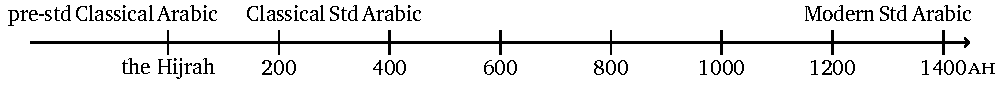
\includegraphics{Learn-Standard-Arabic_files/figure-latex/unnamed-chunk-3-1.pdf}
\caption{\label{fig:unnamed-chunk-3}Timeline of the development of Standard Arabic.}
\end{figure}

In modern times, many new words and meanings have been added to Standard Arabic, often via translation from Western languages, to keep up with technological advancements and modern media.
This modern development of Standard Arabic is called Modern Standard Arabic.
There are also a small amount of words, meanings, and grammatical usages, which existed in Classical Arabic, but which are deemed archaic, and are therefore largely unused, in Modern Standard Arabic.

Figure~1.1 (above) depicts this historical development of Standard Arabic.

\section{Scope of this book}\label{scope-of-this-book}

In this book, we will study Standard Arabic. We will focus on the pre-modern language. If Allāh wills, this will help you to begin to understand the language of the Qurʾān, the Ḥadīt͡h, and Islāmic literature.

If your goal is to learn Modern Standard Arabic, then this book may still be of help because the core language and the grammar are essentially the same. However, you may prefer to study from a resource that focuses on the modern language.

This book does not touch at all upon the modern colloquial dialects that are spoken in the Arab world today.

\section{How to study from this book}\label{how-to-study-from-this-book}

We will start with the Arabic script and present in each chapter a new concept of Arabic grammar, together with examples. We will also give vocabulary for you to memorize and have chapter exercises. Unfortunately, some of the sentences we present, both as examples and as chapter exercises, because of their construction and subject matter, may seem of dubious usefulness to a learner wanting to learn practical usage. We ask that you overlook this and bear with us as we try to reinforce grammatical concepts. In answering the exercises, we strongly recommend that you memorize the vocabulary in full and write down the answers on paper with a pen.

We strongly recommend that you \textbf{not}:

\begin{itemize}
\tightlist
\item
  answer the exercises verbally without writing them down,
\item
  look up the answers before attempting to write the answer yourself,
\item
  look up words in the vocabulary list without memorizing them,
\item
  proceed to the next chapter before memorizing the vocabulary and going through the exercises.
\end{itemize}

Be aware that while Arabic grammar requires effort to master to a proficient degree, the real barrier to reading and understanding Arabic texts by oneself is vocabulary. Arabic is a very rich language and knowledge of a few thousand words is needed before the student can begin to read texts independently.

You may also find yourself having to go back a few chapters every once in a while and revising the concepts therein. This is very normal and not a cause for any alarm. It may also prove beneficial to re-do the exercises of that chapter when this occurs.

\appendix


\chapter{Rules for writing hamzah}\label{hamzarules}

\section{Seats of hamzah}\label{seats-of-hamzah}

Hamzah is written in four different ways:

\begin{enumerate}
\def\labelenumi{\arabic{enumi}.}
\tightlist
\item
  Seated on an \emph{ʾalif}: \foreignlanguage{arabic}{أ} or \foreignlanguage{arabic}{إ}
\item
  Seated on an \emph{wāw}: \foreignlanguage{arabic}{ؤ}
\item
  Seated on an \emph{yāʾ}: \foreignlanguage{arabic}{ئ}
\item
  Unseated: \foreignlanguage{arabic}{ء}
\end{enumerate}

Here are some of notes about writing hamzah in the above four methods:

\begin{itemize}
\item
  When unseated hamzah comes between two letters that are joined, then it is written above the line that joins them, for example: \foreignlanguage{arabic}{خَطِيءَة} \emph{k͡haṭīʾah}. In this word, the \emph{yāʾ} \foreignlanguage{arabic}{ي} joins to the \emph{tāʾ marbūṭah} \foreignlanguage{arabic}{ة}.
\item
  When unseated hamzah is followed by an \emph{ʾalif}: \foreignlanguage{arabic}{ءا}, the combination of hamzah and \emph{ʾalif} is usually written as \foreignlanguage{arabic}{آ} as a convention. Examples: \foreignlanguage{arabic}{آمَنَ} \emph{ʾāmana}, \foreignlanguage{arabic}{ظَمْآن} \emph{ḍ͡hamʾān}, \foreignlanguage{arabic}{شَنَآن} \emph{s͡hanaʾān}. However, when the \emph{ʾalif} is a suffix or part of a suffix, or the hamzah is doubled, or there is an \emph{ʾalif} before the hamzah then we will write \foreignlanguage{arabic}{ءا}, not \foreignlanguage{arabic}{آ}. Examples: \foreignlanguage{arabic}{شَيْءَانِ} \emph{s͡hayʾāni}, \foreignlanguage{arabic}{سَءَّال} \emph{saʾʾāl}, \foreignlanguage{arabic}{قِرَاءَات} \emph{qirāʾāt}.
\item
  When hamzah is seated on \emph{ʾalif}, if it has an \emph{kasrah}, it is written below the \emph{ʾalif}: \foreignlanguage{arabic}{إِ}. Otherwise, it is written above the \emph{ʾalif}: \foreignlanguage{arabic}{أَ}, \foreignlanguage{arabic}{أُ}, \foreignlanguage{arabic}{أْ}.
\item
  When hamzah is seated on \emph{yāʾ} \foreignlanguage{arabic}{ئ} the dots of the \emph{yāʾ} are no longer written. Here's how it will appear in different positions:

  \begin{longtable}[]{@{}llll@{}}
  \toprule\noalign{}
  Isolated & End & Middle & Beginnning \\
  \midrule\noalign{}
  \endhead
  \bottomrule\noalign{}
  \endlastfoot
  \foreignlanguage{arabic}{ئ} & \foreignlanguage{arabic}{ـئ} & \foreignlanguage{arabic}{ـئـ} & \foreignlanguage{arabic}{ئـ} \\
  \end{longtable}

  Note that hamzah is seated on \emph{yāʾ} in the middle position \foreignlanguage{arabic}{ـئـ} is different from unseated hamzah between two joining letters \foreignlanguage{arabic}{ـءـ}.
\end{itemize}

So how do we know when to write hamzah unseated and when seated? And how do we choose between its three different seats? There are a set of rules that we need to follow in order to correctly write hamzah. Before we give the rules we will first present the underlying principle behind the rules.

\section{Rules for determining the seat of hamzah}\label{rules-for-determining-the-seat-of-hamzah}

\subsection{Separate main word from prefixes and suffixes}\label{separate-main-word-from-prefixes-and-suffixes}

In order to determine the seat of hamzah for a words, we must first separate the main word from any prefixes and suffixes.
We will determine the seat of hamzah for the main word first.
Hamzah can occur in three positions in the main word:

\begin{enumerate}
\def\labelenumi{\arabic{enumi}.}
\tightlist
\item
  At the beginning of the word
\item
  In the middle of the word
\item
  At the end of the word
\end{enumerate}

We will treat each of these positions below.

\subsubsection{At the beginning of the word}\label{at-the-beginning-of-the-word}

When hamzah occurs in the beginning of a word, then:

\begin{enumerate}
\def\labelenumi{\alph{enumi}.}
\tightlist
\item
  If the hamzah carries a long-\emph{ā} vowel, it is written unseated followed by an \emph{ʾalif} and written as \foreignlanguage{arabic}{آ}, for example \foreignlanguage{arabic}{آمَنَ} \emph{ʾāmana}.
\item
  If the hamzah carries any other vowel, it is written seated on an \emph{ʾalif}, and is marked with the appropriated vowel mark, for example \foreignlanguage{arabic}{أَسْلَمَ} \emph{ʾaslama}, \foreignlanguage{arabic}{أُرِيدُ} \emph{ʾurīdu}, \foreignlanguage{arabic}{إِسْلَام} \emph{ʾislām}, \foreignlanguage{arabic}{إِيمَان} \emph{ʾīmān}, \foreignlanguage{arabic}{أُوخِذَ} \emph{ʾūk͡hid͡ha}.
\end{enumerate}

\subsubsection{In the middle of the word}\label{in-the-middle-of-the-word}

The most general case is when hamzah is in the middle of a word.

Arabic has three short vowels, three long vowels, two diphthongs, and a \emph{sukūn}. Each of these has an order of precedence and a hamzah seat.

\begin{longtable}[]{@{}llll@{}}
\toprule\noalign{}
Precedence & Vowel & Seat & \\
\midrule\noalign{}
\endhead
\bottomrule\noalign{}
\endlastfoot
1. & \emph{ī}/\emph{ay} & \foreignlanguage{arabic}{ء} & \\
2. & \emph{i} & \foreignlanguage{arabic}{ئ} & \\
3. & \emph{ū}/\emph{aw} & \foreignlanguage{arabic}{ء} & \\
4. & \emph{u} & \foreignlanguage{arabic}{ؤ} & \\
5. & \emph{ā} & \foreignlanguage{arabic}{ء} & \\
6. & \emph{a} & \foreignlanguage{arabic}{أ} & \\
7. & \foreignlanguage{arabic}{◌ْ} & \foreignlanguage{arabic}{ء} & \\
\end{longtable}

\textbf{Main rule:} Disregard any doubling mark \foreignlanguage{arabic}{◌ّ} and consider the vowel on the consonant before the hamzah and the \emph{shortened} vowel on the hamzah itself. Determine which of the two vowels wins by being higher in precedence in the above table. The winning vowel's seat will be the seat of the hamzah.

\textbf{Sub-rule:} If the main rule determines that hamzah is to be seated on \emph{ʾalif}, and there is a long \emph{ā} vowel on the hamzah using an \emph{ʾalif}, then hamzah shall be unseated. And the combination of \foreignlanguage{arabic}{ءَا} will usually be written as \foreignlanguage{arabic}{آ}.

Examples:

\begin{longtable}[]{@{}
  >{\raggedright\arraybackslash}p{(\columnwidth - 8\tabcolsep) * \real{0.3158}}
  >{\raggedright\arraybackslash}p{(\columnwidth - 8\tabcolsep) * \real{0.1053}}
  >{\raggedright\arraybackslash}p{(\columnwidth - 8\tabcolsep) * \real{0.1053}}
  >{\raggedright\arraybackslash}p{(\columnwidth - 8\tabcolsep) * \real{0.1053}}
  >{\raggedright\arraybackslash}p{(\columnwidth - 8\tabcolsep) * \real{0.3684}}@{}}
\toprule\noalign{}
\begin{minipage}[b]{\linewidth}\raggedright
Word
\end{minipage} & \begin{minipage}[b]{\linewidth}\raggedright
Vowel on consonant before hamzah
\end{minipage} & \begin{minipage}[b]{\linewidth}\raggedright
Shortened vowel on hamzah
\end{minipage} & \begin{minipage}[b]{\linewidth}\raggedright
Winning vowel
\end{minipage} & \begin{minipage}[b]{\linewidth}\raggedright
Seated hamzah
\end{minipage} \\
\midrule\noalign{}
\endhead
\bottomrule\noalign{}
\endlastfoot
\foreignlanguage{arabic}{هَيْءَة} \emph{hayʾah} & \emph{ay} & \emph{a} & \emph{ay} & \foreignlanguage{arabic}{ء} \\
{\tradarab{خَطِيءَة}} \emph{k͡haṭīʾah} & \emph{ī} & \emph{a} & \emph{ī} & \foreignlanguage{arabic}{ء} \\
\foreignlanguage{arabic}{اسْتِيءَاس} \emph{ʾistīʾās} & \emph{ī} & \emph{a} & \emph{ī} & \foreignlanguage{arabic}{ء} (Exception: \foreignlanguage{arabic}{ءَا} is not written as \foreignlanguage{arabic}{آ} when the preceding vowel is \emph{ī}.) \\
\foreignlanguage{arabic}{تَوْءَم} \emph{tawʾam} & \emph{aw} & \emph{a} & \emph{aw} & \foreignlanguage{arabic}{ء} \\
\foreignlanguage{arabic}{سَائِل} \emph{sāʾil} & \emph{ā} & \emph{i} & \emph{i} & \foreignlanguage{arabic}{ئ} \\
\foreignlanguage{arabic}{تَسَاؤُل} \emph{tasāʾul} & \emph{ā} & \emph{u} & \emph{u} & \foreignlanguage{arabic}{ؤ} \\
\foreignlanguage{arabic}{تَسَاءَلَ} \emph{tasāʾala} & \emph{ā} & \emph{a} & \emph{ā} & \foreignlanguage{arabic}{ء} \\
\foreignlanguage{arabic}{قِرَاءَات} \emph{qirāʾāt} & \emph{ā} & \emph{a} & \emph{ā} & \foreignlanguage{arabic}{ء} \\
\foreignlanguage{arabic}{مَسْؤُول} \emph{masʾūl} & \foreignlanguage{arabic}{◌ْ} & \emph{u} & \emph{u} & \foreignlanguage{arabic}{ؤ} \\
\foreignlanguage{arabic}{تَرْئِيس} \emph{tarʾīs} & \foreignlanguage{arabic}{◌ْ} & \emph{i} & \emph{i} & \foreignlanguage{arabic}{ئ} \\
\foreignlanguage{arabic}{مِرْآة} \emph{mirʾāh} & \foreignlanguage{arabic}{◌ْ} & \emph{a} & \emph{a} & \foreignlanguage{arabic}{ء} (Using sub-rule.) \\
\foreignlanguage{arabic}{ظَمْآن} \emph{ḍ͡hamʾān} & \foreignlanguage{arabic}{◌ْ} & \emph{a} & \emph{a} & \foreignlanguage{arabic}{ء} (Using sub-rule.) \\
\foreignlanguage{arabic}{مَسْأَلَة} \emph{masʾalah} & \foreignlanguage{arabic}{◌ْ} & \emph{a} & \emph{a} & \foreignlanguage{arabic}{أ} \\
\foreignlanguage{arabic}{الْمَرْأَة} \emph{almarʾah} & \foreignlanguage{arabic}{◌ْ} & \emph{a} & \emph{a} & \foreignlanguage{arabic}{أ} \\
\foreignlanguage{arabic}{بِئْسَ} \emph{biʾsa} & \emph{i} & \foreignlanguage{arabic}{◌ْ} & \emph{i} & \foreignlanguage{arabic}{ئ} \\
\foreignlanguage{arabic}{سُؤْلَکَ} \emph{suʾlaka} & \emph{u} & \foreignlanguage{arabic}{◌ْ} & \emph{u} & \foreignlanguage{arabic}{ؤ} \\
\foreignlanguage{arabic}{کَأْس} \emph{kaʾs} & \emph{a} & \foreignlanguage{arabic}{◌ْ} & \emph{a} & \foreignlanguage{arabic}{أ} \\
\foreignlanguage{arabic}{سُئِلَ} \emph{suʾila} & \emph{u} & \emph{i} & \emph{i} & \foreignlanguage{arabic}{ئ} \\
\foreignlanguage{arabic}{يَئِسَ} \emph{yaʾisa} & \emph{a} & \emph{i} & \emph{i} & \foreignlanguage{arabic}{ئ} \\
\foreignlanguage{arabic}{رَئِيس} \emph{raʾīs} & \emph{a} & \emph{i} & \emph{i} & \foreignlanguage{arabic}{ئ} \\
\foreignlanguage{arabic}{سُؤَال} \emph{suʾāl} & \emph{u} & \emph{a} & \emph{u} & \foreignlanguage{arabic}{ؤ} \\
\foreignlanguage{arabic}{رُؤُوس} \emph{ruʾūs} & \emph{u} & \emph{u} & \emph{u} & \foreignlanguage{arabic}{ؤ} \\
\foreignlanguage{arabic}{لُؤَيّ} \emph{luʾayy} & \emph{u} & \emph{a} & \emph{u} & \foreignlanguage{arabic}{ؤ} \\
\foreignlanguage{arabic}{شَنَآن} \emph{s͡hanaʾān} & \emph{a} & \emph{a} & \emph{a} & \foreignlanguage{arabic}{ء} (Using sub-rule.) \\
\foreignlanguage{arabic}{سَأَلَ} \emph{saʾala} & \emph{a} & \emph{a} & \emph{a} & \foreignlanguage{arabic}{أ} \\
\foreignlanguage{arabic}{رَأَىٰ} \emph{raʾā} & \emph{a} & \emph{a} & \emph{a} & \foreignlanguage{arabic}{أ} \\
\foreignlanguage{arabic}{رَأَّسَ} \emph{raʾʾasa} & \emph{a} & \emph{a} & \emph{a} & \foreignlanguage{arabic}{أ} \\
\foreignlanguage{arabic}{يُرَئِّسُ} \emph{yuraʾʾisu} & \emph{a} & \emph{i} & \emph{i} & \foreignlanguage{arabic}{ئ} \\
\foreignlanguage{arabic}{رُئِّسَ} \emph{ruʾʾisa} & \emph{u} & \emph{i} & \emph{i} & \foreignlanguage{arabic}{ئ} \\
\foreignlanguage{arabic}{تَفَؤُّل} \emph{tafaʾʾul} & \emph{a} & \emph{u} & \emph{u} & \foreignlanguage{arabic}{ؤ} \\
\foreignlanguage{arabic}{سَءَّال} \emph{saʾʾāl} & \emph{a} & \emph{a} & \emph{a} & \foreignlanguage{arabic}{ء} (Using sub-rule.) \\
\foreignlanguage{arabic}{لَءَّال} \emph{laʾʾāl} & \emph{a} & \emph{a} & \emph{a} & \foreignlanguage{arabic}{ء} (Using sub-rule.) \\
\end{longtable}

\subsubsection{At the end of the word}\label{at-the-end-of-the-word}

When hamzah occurs at the end of a word, disregard the vowel on hamzah itself, and consider only the vowel on preceding consonant.
Plug it into the table as above, and determine to determine the seat of hamzah.

\begin{longtable}[]{@{}lll@{}}
\toprule\noalign{}
Word & Vowel on consonant before hamzah & Seated hamzah \\
\midrule\noalign{}
\endhead
\bottomrule\noalign{}
\endlastfoot
\foreignlanguage{arabic}{دُعَاءُ} \emph{duɛāʾu} & \emph{ā} & \foreignlanguage{arabic}{ء} \\
\foreignlanguage{arabic}{سُوءُ} \emph{sūʾu} & \emph{ū} & \foreignlanguage{arabic}{ء} \\
\foreignlanguage{arabic}{جِيءَ} \emph{jīʾa} & \emph{ī} & \foreignlanguage{arabic}{ء} \\
\foreignlanguage{arabic}{ضَوْءَ} \emph{ḍawʾa} & \emph{aw} & \foreignlanguage{arabic}{ء} \\
\foreignlanguage{arabic}{شَيْءَ} \emph{s͡hayʾa} & \emph{ay} & \foreignlanguage{arabic}{ء} \\
\foreignlanguage{arabic}{بُطْءُ} \emph{buṭʾu} & \foreignlanguage{arabic}{◌ْ} & \foreignlanguage{arabic}{ء} \\
\foreignlanguage{arabic}{عِبْءُ} \emph{ɛibʾu} & \foreignlanguage{arabic}{◌ْ} & \foreignlanguage{arabic}{ء} \\
\foreignlanguage{arabic}{شَطْءُ} \emph{s͡haṭʾu} & \foreignlanguage{arabic}{◌ْ} & \foreignlanguage{arabic}{ء} \\
\foreignlanguage{arabic}{يُهَدِّئُ} \emph{yuhaddiʾu} & \emph{i} & \foreignlanguage{arabic}{ئ} \\
\foreignlanguage{arabic}{سَيِّئُ} \emph{sayyiʾu} & \emph{i} & \foreignlanguage{arabic}{ئ} \\
\foreignlanguage{arabic}{بَطُؤَ} \emph{baṭuʾa} & \emph{u} & \foreignlanguage{arabic}{ؤ} \\
\foreignlanguage{arabic}{يَهْدَأُ} \emph{yahdaʾu} & \emph{a} & \foreignlanguage{arabic}{أ} \\
\foreignlanguage{arabic}{مُبْتَدَإِ} \emph{mubtadaʾi} & \emph{a} & \foreignlanguage{arabic}{إ} \\
\end{longtable}

The exception to this rule is when the previous letter is a doubled \emph{wāw} with an \emph{ḍammah}.
In this case the hamzah will again be unseated. Example \foreignlanguage{arabic}{تَبَوُّءُ} \emph{tabawwuʾu}.

Note also that \foreignlanguage{arabic}{مُبْتَدَإِ} \emph{mubtadaʾi} can be written with the hamzah below the \emph{ʾalif} because of the \emph{i}-mark on the hamzah.
But it is also common to write it as \foreignlanguage{arabic}{مُبْتَدَأ} \emph{mubtadaʾ}, especially when the hamzah is unvoweled.

\subsection{Prefixes and suffixes}\label{prefixes-and-suffixes}

\subsubsection{Prefixes}\label{prefixes}

If hamzah is in the beginning of a word, adding a prefix to the word will not alter the writing of the hamzah. Examples:

\begin{itemize}
\tightlist
\item
  \foreignlanguage{arabic}{لِ + أُسْتَاذِ = لِأُسْتَاذِ}\\
\item
  \foreignlanguage{arabic}{الْ + آخِرَة = الْآخِرَة}
\end{itemize}

\subsubsection{Suffixes}\label{suffixes}

If hamzah is at the end of a word, adding a suffix to the word can, in general, alter the writing of the hamzah.
Hamzah is now, generally, treated as if it is in the middle of the word, and the rules for hamzah in the middle of a word apply.
Examples:

\begin{longtable}[]{@{}
  >{\raggedright\arraybackslash}p{(\columnwidth - 8\tabcolsep) * \real{0.3158}}
  >{\raggedright\arraybackslash}p{(\columnwidth - 8\tabcolsep) * \real{0.1053}}
  >{\raggedright\arraybackslash}p{(\columnwidth - 8\tabcolsep) * \real{0.1053}}
  >{\raggedright\arraybackslash}p{(\columnwidth - 8\tabcolsep) * \real{0.1053}}
  >{\raggedright\arraybackslash}p{(\columnwidth - 8\tabcolsep) * \real{0.3684}}@{}}
\toprule\noalign{}
\begin{minipage}[b]{\linewidth}\raggedright
Word
\end{minipage} & \begin{minipage}[b]{\linewidth}\raggedright
Vowel on consonant before hamzah
\end{minipage} & \begin{minipage}[b]{\linewidth}\raggedright
Shortened vowel on hamzah
\end{minipage} & \begin{minipage}[b]{\linewidth}\raggedright
Winning vowel
\end{minipage} & \begin{minipage}[b]{\linewidth}\raggedright
Seated hamzah
\end{minipage} \\
\midrule\noalign{}
\endhead
\bottomrule\noalign{}
\endlastfoot
\foreignlanguage{arabic}{بَرِيءُونَ} \emph{barīʾūna} & \emph{ī} & \emph{u} & \emph{ī} & \emph{ء} \\
\foreignlanguage{arabic}{بَرِيءَانِ} \emph{barīʾāni} & \emph{ī} & \emph{a} & \emph{ī} & \emph{ء} \\
\foreignlanguage{arabic}{بَرِيءِينَ} \emph{barīʾīna} & \emph{ī} & \emph{i} & \emph{ī} & \emph{ء} \\
\foreignlanguage{arabic}{بَرِيءَيْنِ} \emph{barīʾayni} & \emph{ī} & \emph{a} & \emph{ī} & \emph{ء} \\
\foreignlanguage{arabic}{شَيْءُهُ} \emph{s͡hayʾuhu} & \emph{ay} & \emph{u} & \emph{ay} & \emph{ء} \\
\foreignlanguage{arabic}{شَيْءَهُ} \emph{s͡hayʾahu} & \emph{ay} & \emph{a} & \emph{ay} & \emph{ء} \\
\foreignlanguage{arabic}{شَيْءِهِ} \emph{s͡hayʾihi} & \emph{ay} & \emph{i} & \emph{ay} & \emph{ء} \\
\foreignlanguage{arabic}{شَيْءَانِ} \emph{s͡hayʾāni} & \emph{ay} & \emph{a} & \emph{ay} & \emph{ء} \\
\foreignlanguage{arabic}{شَيْءَيْنِ} \emph{s͡hayʾayni} & \emph{ay} & \emph{a} & \emph{ay} & \emph{ء} \\
\foreignlanguage{arabic}{مَجِيءُهُ} \emph{majīʾuhu} & \emph{ī} & \emph{u} & \emph{ī} & \emph{ء} \\
\foreignlanguage{arabic}{مَجِيءَهُ} \emph{majīʾahu} & \emph{ī} & \emph{a} & \emph{ī} & \emph{ء} \\
\foreignlanguage{arabic}{مَجِيءِهِ} \emph{majīʾihi} & \emph{ī} & \emph{i} & \emph{ī} & \emph{ء} \\
\foreignlanguage{arabic}{سُوئِهِ} \emph{sūʾihi} & \emph{ū} & \emph{i} & \emph{i} & \emph{ئ} \\
\foreignlanguage{arabic}{ضَوْئِهِ} \emph{ḍawʾihi} & \emph{aw} & \emph{i} & \emph{i} & \emph{ئ} \\
\foreignlanguage{arabic}{سُوءَهُ} \emph{sūʾahu} & \emph{ū} & \emph{a} & \emph{ū} & \emph{ء} \\
\foreignlanguage{arabic}{سُوءَانِ} \emph{sūʾāni} & \emph{ū} & \emph{a} & \emph{ū} & \emph{ء} \\
\foreignlanguage{arabic}{ضَوْءَهُ} \emph{ḍawʾahu} & \emph{aw} & \emph{a} & \emph{aw} & \emph{ء} \\
\foreignlanguage{arabic}{ضَوْءَانِ} \emph{ḍawʾāni} & \emph{aw} & \emph{a} & \emph{aw} & \emph{ء} \\
\foreignlanguage{arabic}{سُوءُهُ} \emph{sūʾuhu} & \emph{ū} & \emph{u} & \emph{ū} & \emph{ء} \\
\foreignlanguage{arabic}{يَسُوءُونَ} \emph{yasūʾūna} & \emph{ū} & \emph{u} & \emph{ū} & \emph{ء} \\
\foreignlanguage{arabic}{نُوآنٌ} \emph{nūʾānun}. & \emph{ū} & \emph{a} & \emph{ū} & \emph{ء} \\
\foreignlanguage{arabic}{مُتَّکِئِينَ} \emph{muttakiʾīna} & \emph{i} & \emph{i} & \emph{i} & \emph{ئ} \\
\foreignlanguage{arabic}{يُبَرِّئُونَ} \emph{yubarriʾūna} & \emph{i} & \emph{u} & \emph{i} & \emph{ئ} \\
\foreignlanguage{arabic}{يُبَرَّؤُونَ} \emph{yubarraʾūna} & \emph{a} & \emph{u} & \emph{u} & \emph{ؤ} \\
\end{longtable}

There are some exceptions:

If the letter before the hamzah has a \emph{sukūn} and is not \emph{wāw} or \emph{yāʾ},
then the hamzah will be written unseated. Examples:

\begin{itemize}
\tightlist
\item
  \foreignlanguage{arabic}{جُزْءَانِ} \emph{juzʾāni}\\
\item
  \foreignlanguage{arabic}{عِبْءَانِ} \emph{ɛibʾāni}\\
\item
  \foreignlanguage{arabic}{عِبْءَيْنِ} \emph{ɛibʾayni}\\
\item
  \foreignlanguage{arabic}{بُطْءَهُ} \emph{buṭʾahu}\\
\item
  \foreignlanguage{arabic}{بُطْءُهُ} \emph{buṭʾuhu}\\
\item
  \foreignlanguage{arabic}{بُطْءِهِ} \emph{buṭʾihi}
\end{itemize}

(\foreignlanguage{arabic}{انِ}, \foreignlanguage{arabic}{يْنِ}, \foreignlanguage{arabic}{هُ}, and \foreignlanguage{arabic}{هِ} are suffixes.)

\subsection{\texorpdfstring{\emph{tanwīn} on final hamzah}{tanwīn on final hamzah}}\label{tanwin-on-final-hamzah}

\emph{tanwīn} on a final hamzah does not affect the writing of the hamzah except in the case of \emph{tanwīn al-fat·ḥ}. When writing \emph{tanwīn al-fat·ḥ} on a hamzah at the end of a word:

\begin{enumerate}
\def\labelenumi{\arabic{enumi}.}
\item
  If there is an \emph{ʾalif} before a unseated hamzah \foreignlanguage{arabic}{اء}, then we don't add a silent \emph{ʾalif} when writing \emph{tanwīn al-fat·ḥ}. For example \foreignlanguage{arabic}{دَاء} becomes \foreignlanguage{arabic}{دَاءً} \emph{dāʾan}, not \foreignlanguage{arabic}{دَاءًا}.
\item
  Otherwise, we add the silent \emph{ʾalif} after the hamzah so that the hamzah is now in the middle of the word with a suffix \emph{ʾalif} after it. We now pretend that the hamzah has an \emph{fat·ḥah} and that the \emph{ʾalif} after it is a long-\emph{ā} vowel. Then we go through the rules for writing hamzah in the middle of a word (given above) to determine how hamzah will be written. We then write the \emph{an}-mark on the hamzah. Examples:
\end{enumerate}

\begin{itemize}
\tightlist
\item
  \foreignlanguage{arabic}{مُبْتَدَأ} becomes \foreignlanguage{arabic}{مُبْتَدَأٌ، مُبْتَدَءًا، مُبْتَدَإٍ}
\item
  \foreignlanguage{arabic}{مَلْجَأ} becomes \foreignlanguage{arabic}{مَلْجَأٌ، مَلْجَءًا، مَلْجَإٍ}
\item
  \foreignlanguage{arabic}{جُزْء} becomes \foreignlanguage{arabic}{جُزْءٌ، جُزْءًا، جُزْءٍ}
\item
  \foreignlanguage{arabic}{شَيْء} becomes \foreignlanguage{arabic}{شَيْءٌ، شَيْءًا، شَيْءٍ}
\end{itemize}

\subsection{Variants}\label{variants}

There are some historical and regional variants to the above rules. The main one is a variant of rule 2.b.ii above. In this variant, when the letter before hamzah has a \emph{sukūn}, the hamzah is generally written unseated. So they write:

\begin{itemize}
\tightlist
\item
  \foreignlanguage{arabic}{مَسْءُول} instead of \foreignlanguage{arabic}{مَسْؤُول}
\item
  \foreignlanguage{arabic}{أَسْءِلَة} instead of \foreignlanguage{arabic}{أَسْئِلَة}
\item
  \foreignlanguage{arabic}{مَسْءَلَة} instead of \foreignlanguage{arabic}{مَسْأَلَة}
\end{itemize}

However, this rule appears to be not consistently followed. For example, \emph{al-nas͡hʾah} is generally always written \foreignlanguage{arabic}{النَّشْأَة} never \foreignlanguage{arabic}{النَّشْءَة}.

A second variant is to avoid the repetition of vowel letters like \foreignlanguage{arabic}{و} and \foreignlanguage{arabic}{ي}. So they write:

\begin{itemize}
\tightlist
\item
  \foreignlanguage{arabic}{رُءُوس} instead of \foreignlanguage{arabic}{رُؤُوس}.
\item
  \foreignlanguage{arabic}{رَءِيس} instead of \foreignlanguage{arabic}{رَئِيس}.
\end{itemize}

\end{document}
